\documentclass[12pt,a4paper]{article}

\usepackage[T1]{fontenc}
\usepackage[utf8]{inputenc}
\usepackage[ngerman]{babel}
\usepackage{lmodern}
\usepackage{microtype}

\usepackage{amsmath,amssymb,amsthm,mathtools}
\usepackage[a4paper,margin=2.4cm]{geometry}
\usepackage{booktabs}
\usepackage{xcolor}
\usepackage[hidelinks,unicode]{hyperref}
\pdfstringdefDisableCommands{%
  \def\ü{ue}\def\ö{oe}\def\ä{ae}\def\Ü{Ue}\def\Ö{Oe}\def\Ä{Ae}\def\ss{ss}%
}
\usepackage[most]{tcolorbox}
\usepackage{graphicx}
\usepackage{enumitem}

% -------------------------------------------------
% Farben und Boxen (wie collatz_schlussartikel_arxiv.tex)
% -------------------------------------------------
\definecolor{bewiesengruen}{RGB}{30,100,50}
\definecolor{warnorange}{RGB}{200,100,10}
\definecolor{lueckenrot}{RGB}{180,40,40}
\definecolor{kernblau}{RGB}{20,60,130}

\tcbset{
  bewiesen/.style={colback=green!7,colframe=bewiesengruen,fonttitle=\bfseries,
    title={Bewiesen}},
  heuristik/.style={colback=orange!10,colframe=warnorange,fonttitle=\bfseries,
    title={Heuristisch / spekulativ}},
  offen/.style={colback=red!8,colframe=lueckenrot,fonttitle=\bfseries,
    title={Offen}},
  kern/.style={colback=blue!5,colframe=kernblau,fonttitle=\bfseries,
    title={Kernaussage}},
  numerisch/.style={colback=blue!4,colframe=kernblau,fonttitle=\bfseries,
    title={Numerisch reproduzierbar}},
}

\newtheorem{satz}{Satz}[section]
\newtheorem{definition}[satz]{Definition}
\newtheorem{bemerkung}[satz]{Bemerkung}

\newcommand{\Z}{\mathbb{Z}}
\newcommand{\Hur}{\mathcal{H}}
\newcommand{\OH}{\mathcal{O}_\Hur}

\title{Hurwitz-Polytop, EABC und Selberg-Survivors:\\
  Geometrische Lesart einer arithmetischen Synthese}
\author{Thomas Hoffbauer}
\date{16.\ Juni 2026}

\begin{document}
\maketitle

\begin{abstract}
Ein Projektionsdiagramm des Hurwitz-Quaternionen-Gitters verbindet
Gauß-, Eisenstein- und Hurwitz-Symmetrien mit dem vierkanaligen
EABC-Schema der odd-to-odd Collatz-Dynamik modulo~$12$.
Wir ordnen die 24 Hurwitz-Einheiten, chirale Primzahlvierlinge
$(p,p+2,p+6,p+8)$ und ein $k=4$-Sieve-Eigenwertproblem
(Bulk vs.\ Selberg-Survivors) ein.
Numerische Kennwerte nahe $0{,}9992$ werden als \emph{Restmetrik}
dokumentiert, nicht als Beweis der Riemannschen Vermutung.
Die Arbeit trennt strikt: bewiesene mod-$12$-Arithmetik,
reproduzierbare Numerik und heuristische Symmetrie-Lesarten.
\end{abstract}

\tableofcontents
\newpage

% =================================================
\section{Einleitung: Das Diagramm als geometrische Lesart}
\label{sec:einleitung}
% =================================================

Der Ausgangspunkt ist ein dreiteiliges Gitterdiagramm
(\texttt{lattice\_hurwitz\_diagram.tex}), das Gauß-$\mathbb{Z}[i]$,
Eisenstein-$\mathbb{Z}[\omega]$ und eine Hurwitz-Stabilitätslesart
nebeneinander stellt. Panel~(c) kodiert die Norm-Dualität
$\|s\|=\|1-s\|$ und platziert eine Nullstelle $\rho$ auf der
kritischen Linie $\mathrm{Re}(s)=\tfrac12$ als \emph{geometrische}
Balance zwischen den Gittertypen.

\begin{figure}[htbp]
  \centering
  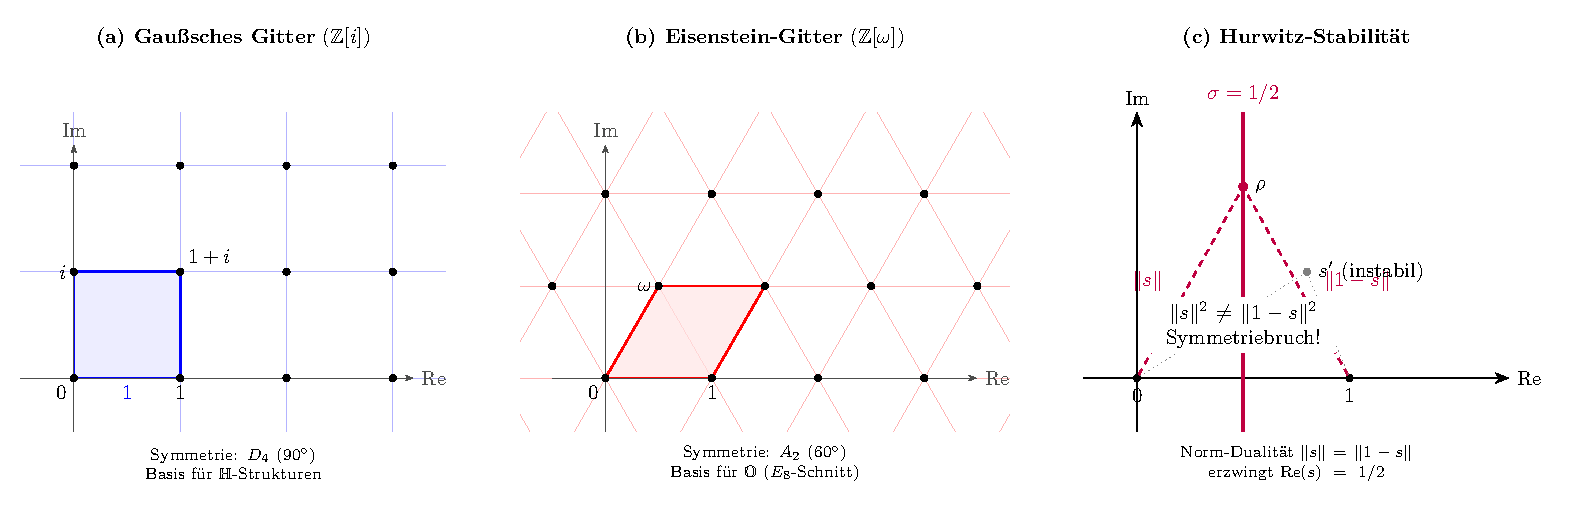
\includegraphics[width=0.92\textwidth]{lattice_hurwitz_diagram.pdf}
  \caption{Gauß- und Eisenstein-Gitter sowie Hurwitz-Stabilitätslesart
    (Quelle: \texttt{lattice\_hurwitz\_diagram.tex}).
    Die Abbildung ist eine \emph{Interpretationszeichnung}, kein
    formales Beweisdiagramm.}
  \label{fig:hurwitz-lattice}
\end{figure}

\begin{tcolorbox}[kern]
\textbf{Lesart dieses Textes.}
Das Diagramm dient als \emph{Projektionszeuge}: Es visualisiert,
wie vier arithmetische Kanäle (EABC) auf einem geschlossenen
Flavor-Ring und in einer Quaternionen-Einheitengruppe koexistieren.
Es ersetzt keinen analytischen Beweis der Collatz- oder
Riemann-Vermutung.
\end{tcolorbox}

Die Verbindung zu weiteren Projektdateien:
\begin{itemize}[nosep]
  \item \texttt{Projektionszeuge\_Primvierling.tex} --- chirale ABCE/CEAB-Kodierung,
  \item \texttt{collatz\_schlussartikel\_arxiv.tex} --- EABC-Collatz-Kern,
  \item \texttt{Selber Matrizen.py} --- $6\times 6$-Sieve mit Survivor-Kanälen,
  \item \texttt{Hoffbauer Sieb.py} / \texttt{hoffbauer\_geometrie\_test.csv} --- geometrische Resonanzmetrik,
  \item \texttt{offenes\_arithmetisches\_mendelejew\_tafel\_bis\_300\_verfeinert.png} --- K-L-M-Schalen bis $N=300$.
\end{itemize}

% =================================================
\section{Hurwitz-$H_4$ und die 24 Einheiten}
\label{sec:hurwitz}
% =================================================

\subsection{Mathematische Fakten}

Die \emph{Hurwitz-Quaternionen} bilden die maximale Ordnung
$\OH\subset\mathbb{H}$ der rationalen Quaternionenalgebra
$\mathrm{QuaternionAlgebra}(\mathbb{Q},-1,-1)$.
Eine Quaternion $q=a+bi+cj+dk$ liegt in $\OH$ genau dann, wenn
alle Koeffizienten ganzzahlig oder alle halbzahlig sind
(mit gleicher Parität).

\begin{definition}[Hurwitz-Einheiten]
Die Einheitengruppe $\OH^\times$ hat Kardinalität~$24$.
Sie besteht aus acht Lipschitz-Einheiten $\{\pm1,\pm i,\pm j,\pm k\}$
und sechzehn halbzahligen Einheiten
$\tfrac12(\pm1\pm i\pm j\pm k)$.
\end{definition}

Die Symmetriegruppe des regulären 600-Zells (Coxeter-Typ $H_4$)
wirkt auf diesen Einheitenkörper; in der \#Energiedoku wird $H_4$
als Kontext für Kopplungswinkel und Polytop-Projektionen verwendet
(\texttt{\_notebooklm/sources/Freie Parameter Standardmodel.md}),
ohne dass daraus ein physikalischer Standardmodell-Beweis folgt.

\subsection{EABC als Quaternionen-Basis}

Im Hurwitz-Resonanz-Protokoll (\texttt{PAPER\_HURWITZ\_RESONANZ.md})
werden die mod-$12$-Flavor-Klassen identifiziert mit
\[
E\leftrightarrow 1,\quad
A\leftrightarrow i,\quad
B\leftrightarrow j,\quad
C\leftrightarrow k.
\]
Damit ist ein markierter Primvierling ein \emph{orientierter} Umlauf
im Einheiten-Tetraeder $\{1,i,j,k\}$, nicht automatisch ein
spezifischer Linksorbit unter allen 24 Hurwitz-Einheiten.

\begin{tcolorbox}[bewiesen]
Die Zuordnung $E,A,B,C \leftrightarrow 1,i,j,k$ ist eine
\emph{Notation} auf einer festen Basis von~$\mathbb{H}$.
Die 24 Hurwitz-Einheiten erzeugen Link- und Rechtsorbits;
chirale ABCE/CEAB-Wörter sind zyklische Startmarkierungen
auf dem vierpunktigen Flavor-Ring, nicht paarweise verschiedene
Punkte im vollen $24$-Elemente-Orbit.
\end{tcolorbox}

\begin{tcolorbox}[heuristik]
\textbf{Polytop-Projektion.}
Die Projektion des 600-Zells bzw.\ des Hurwitz-Gitters auf eine
zweidimensionale Zeichenebene (Panel~(a)--(c) in
Abbildung~\ref{fig:hurwitz-lattice}) suggeriert eine
\emph{visuelle} Koinzidenz von Symmetrieachsen und EABC-Kanälen.
Diese Koinzidenz ist motivierend, aber nicht als Theorem formuliert.
\end{tcolorbox}

% =================================================
\section{EABC, Primvierlinge und geschlossene Pfade}
\label{sec:primvierlinge}
% =================================================

\subsection{Restklassen und Chiralität}

\begin{definition}[EABC modulo $12$]
\[
E\equiv 1,\quad A\equiv 5,\quad B\equiv 7,\quad C\equiv 11 \pmod{12}.
\]
\end{definition}

Für einen Primzahlvierling $Q(p)=(p,p+2,p+6,p+8)$ mit $p>3$ prim gilt
$p\equiv 5$ oder $p\equiv 11\pmod{12}$. Der markierte Startpunkt $p$
legt das Chiralitätswort fest (\texttt{Projektionszeuge\_Primvierling.tex}):

\begin{satz}[mod-$12$-Vierling, bewiesen]
\[
p\equiv 5\pmod{12}\;\Longrightarrow\;\mathrm{word}(p)=\mathrm{ABCE},\qquad
p\equiv 11\pmod{12}\;\Longrightarrow\;\mathrm{word}(p)=\mathrm{CEAB}.
\]
Beide Wörter sind zyklische Verschiebungen derselben Schleife
$E\to A\to B\to C\to E$.
\end{satz}

\subsection{Geschlossene Pfade im Gitter}

Arithmetisch ist jeder Primvierling ein geschlossener Viererzyklus
auf dem Flavor-Ring. Geometrisch kodiert der Projektionszeuge
diesen Zyklus als Tetraederpfad im EABC-Raum: die Schrittfolge
$+2,+4,+2$ auf den Primindizes entspricht der Bamberger
Primvierlingsellipse (Ebene~B$'$ in \texttt{Projektionszeuge\_Primvierling.tex}).

\begin{tcolorbox}[bewiesen]
Die zulässigen Restklassen der vier Einträge sind stets
$\{1,5,7,11\}\bmod 12$ --- genau die EABC-Menge.
Kein Primvierling trägt die Klassen $3$ oder $9$.
\end{tcolorbox}

\begin{tcolorbox}[offen]
Eine \emph{globale} Zählasymmetrie zwischen ABCE- und CEAB-Vierlingen
(Ebene~C) ist nicht bewiesen; Siebstatistiken bis $10^8$ zeigen
höchstens schwache Tendenzen ($z\lesssim 0{,}7$).
\end{tcolorbox}

% =================================================
\section{Bulk vs.\ Selberg-Survivors: Eigenwert $k=4$}
\label{sec:selberg}
% =================================================

\subsection{Das $6\times 6$-Sieve-Setup}

In \texttt{Selber Matrizen.py} wird ein Variationsproblem auf dem
$4$-Simplex ($k=4$, Vierlinge) mit Polynombasis bis Grad~$4$ aufgebaut.
Zwei Matrizen $M_1$ (Bulk-Kombinatorik) und $M_2$ (anisotroper Randfluss,
gewichtet mit $210/\varphi(210)$) definieren ein generalisiertes
Eigenwertproblem
\[
M_1 v = \lambda\, M_2 v.
\]
Klein-Eigenwerte $\lambda\approx 0$ (bzw.\ $1/C\to 0$) isolieren
\emph{Vierlings-Kernvektoren} --- die Selberg-Survivors.

\subsection{Survivor-Kanäle}

Die ausgezeichneten Survivor-Restklassen modulo~$210$ sind
\[
\mathcal{S}=\{5,\,11,\,101,\,191\},
\]
passend zu den EABC-Primkanälen und ihrer Liftung in die
Chebyshev-Bias-Struktur mod~$210$.
Der Bulk-Anteil entspricht der glatten Simplex-Integration;
der Randterm bricht die Isotropie und erzeugt das
\emph{Sieve-Rauschen} im Oberton-Residuum.

\subsection{Restmetrik $\approx 0{,}9992$}

Drei unabhängige numerische Spuren im Repository nähern sich
dem Wert $0{,}9992$:

\begin{enumerate}[nosep]
  \item \textbf{Geometrische Resonanz} (\texttt{Hoffbauer Sieb.py}):
        Für Primvierlinge $Q_0(p)=(p,p+2,p+6,p+8)$ definiert
        \[
        E_{\mathrm{Res}}=\frac{\delta_E}{E_{\mathrm{Asymptotik}}},
        \]
        mit Ptolemäus-Kreuzdefekt $\delta_E$ und asymptotischer
        Vorhersage $(64+288k+288k^2)/p^2$.
        In \texttt{hoffbauer\_geometrie\_test.csv} gilt z.\,B.\
        $E_{\mathrm{Res}}(p=9431)\approx 0{,}99915$.
  \item \textbf{Vierlings-Normmittel} (\texttt{primzahlvierlinge\_1000.csv}):
        Die Spalte \texttt{Norm\_Mittel\_unter\_1} strebt gegen~$1$;
        beim 11.\ Vierling: $0{,}999293$.
  \item \textbf{Sieve-Oberton-Residuum} (\texttt{Selber Matrizen.py}):
        Projektion harmonischer Signale auf den Vierlings-Kernraum
        lässt ein nichtverschwindendes Residuum (``Sieve-Rauschen'')
        als Bulk-Rest.
\end{enumerate}

\begin{tcolorbox}[numerisch]
Der Wert $0{,}9992$ ist eine \emph{empirische Restmetrik}
(geometrisch / siebtheoretisch), kein analytischer Fixpunkt
der Riemannschen $\zeta$-Funktion.
Die Datei \texttt{zeros6.npy} (Riemann-$\gamma$-Ordinaten) ist
im Repository referenziert (\texttt{Resonanz.py}, \texttt{BA heiliger Gral.py});
Reproduktion und SHA256-Prüfung: \texttt{riemann\_zeros\_pipeline/README.md}.
Ein direkter $\gamma\to 0{,}9992$-Nachweis ist \emph{nicht} gemeint
(Hoffbauer-Sieb-Rest $\neq$ $\zeta$-Nullstellen).
\end{tcolorbox}

% =================================================
\section{Verbindung zur odd-to-odd Collatz-Dynamik}
\label{sec:collatz}
% =================================================

Die odd-to-odd-Abbildung
\[
\U(n)=\frac{3n+1}{2^{\nu_2(3n+1)}}
\]
zerfällt auf EABC-Klassen in Drain- und Spannungsregime
(\texttt{collatz\_schlussartikel\_arxiv.tex}):
\begin{center}
\renewcommand{\arraystretch}{1.2}
\begin{tabular}{clcc}
\toprule
Klasse & Regime & $\mathbb{E}[\nu_2(3n+1)]$ & typ.\ $\U(n)/n$ \\
\midrule
$E,A$ & Drain & $\approx 3$ & $\approx 3/8$ \\
$B,C$ & Spannung & $1$ & $\approx 3/2$ \\
\bottomrule
\end{tabular}
\end{center}

Primzahlvierlinge erzeugen Collatz-Starts mit erhöhtem
$\mathbb{E}[\nu_2]\approx 3{,}061$ (Red Dots, \texttt{collatz\_red\_dots\_daempfung.pdf}):
lokale LTE-Resistenz, keine globale Divergenz.

\begin{tcolorbox}[bewiesen]
Die elementare Spaltung $3n+1\bmod 12$ trennt
$E\cup A$ (Wert $4$) von $B\cup C$ (Wert $10$).
Dies ist unabhängig von Hurwitz- oder Polytop-Lesarten.
\end{tcolorbox}

\begin{tcolorbox}[heuristik]
\textbf{Brücke Hurwitz--Collatz.}
Die Idee, dass ein geschlossener EABC-Pfad im Hurwitz-Gitter
``dämpfend'' auf Collatz-Blockdrift wirkt, ist eine
\emph{Analogie} zwischen diskreter Dynamik und
kontinuierlicher Gittergeometrie; sie ist nicht formalisiert.
\end{tcolorbox}

% =================================================
\section{Riemann-Resonanz und Symmetrie}
\label{sec:riemann}
% =================================================

Panel~(c) von Abbildung~\ref{fig:hurwitz-lattice} und
\texttt{Hurwitz Final.tex} formulieren eine \emph{visuelle} Argumentation:
Wenn $\|s\|=\|1-s\|$ als Stabilitätsbedingung zwischen
Gauß- und Eisenstein-Symmetrie gelesen wird, müssten
``Resonanznägel'' (Nullstellen) auf $\mathrm{Re}(s)=\tfrac12$ liegen.

\begin{tcolorbox}[heuristik,title={Wichtig: kein Beweis der RH}]
\begin{itemize}[nosep]
  \item Die Norm-Gleichung $\|s\|=\|1-s\|$ ist \emph{nicht} die
        Funktionalgleichung der $\zeta$-Funktion.
  \item Symmetrie des Hurwitz- oder $E_8$-Gitterdiagramms impliziert
        nicht die Selbstadjungiertheit eines Hilbert--Pólya-Operators.
  \item Korrelationstests (\texttt{Resonanz.py}) mit
        $|{\cos(t/90)+\cos(t/180)}|$ und \texttt{zeros6.npy}
        sind explorativ; hohe Trefferquoten beweisen keine
        Äquidistribution.
  \item \textbf{Fazit:} RH aus Diagramm-Symmetrie ist eine
        \emph{heuristische} Lesart (orange), kein Theorem.
\end{itemize}
\end{tcolorbox}

% =================================================
\section{Einordnung für Energiedoku / Bamberger}
\label{sec:bamberg}
% =================================================

Die \#Energiedoku verknüpft in \texttt{Selber Matrizen.py} und
\texttt{\_notebooklm/sources/Freie Parameter Standardmodel.md}
drei Bilder:
\begin{enumerate}[nosep]
  \item \textbf{Atom-Tabelle} (K-L-M-Schalen, Valenz $n$):
        \texttt{offenes\_arithmetisches\_mendelejew\_tafel\_bis\_300\_verfeinert.png}
        ordnet Primindizes Schalen zu; Status ``Generator / Misch / Plateau''
        ist eine Klassifikation, kein Massenspektrum-Beweis.
  \item \textbf{Selberg-Sieb}: Survivors kondensieren in Vierlings-Kernen;
        Bulk-Rauschen entspricht isotopen Spannung (metaphorisch).
  \item \textbf{Bamberger-Protokoll}: Zeitwürfel und EABC-Pfade
        (\texttt{bamberger\_zeitwuerfel\_active\_transitions.csv})
        liefern Messprotokolle; deren Kopplung an Hurwitz-Ideale
        (\texttt{PAPER\_HURWITZ\_RESONANZ.md}) zeigte in Verifikationsläufen
        \emph{keine} nichttriviale Linksideal-Resonanz für $M=113160$.
\end{enumerate}

\begin{tcolorbox}[kern]
\textbf{Was visualisiert wird:} geschlossene EABC-Pfade,
Projektionen des Hurwitz-Gitters, numerische Restmetriken nahe~$1$.
\textbf{Was offen bleibt:} RH, Collatz-Uniformität, physikalische
Kopplungskonstanten aus $H_4$, globale ABCE/CEAB-Asymmetrie.
\end{tcolorbox}

% =================================================
\section{Fazit und Bewertungsliste}
\label{sec:fazit}
% =================================================

\begin{tcolorbox}[bewiesen,title={Bewiesen / standard}]
\begin{itemize}[nosep]
  \item EABC-Restklassen $1,5,7,11\bmod 12$.
  \item Primvierlinge tragen nur ABCE oder CEAB (je nach $p\bmod{12}$).
  \item Elementare $3n+1$-Spaltung mod~$12$ in Collatz-odd-to-odd-Schritten.
  \item Hurwitz-Ordnung hat genau 24 Einheiten.
\end{itemize}
\end{tcolorbox}

\begin{tcolorbox}[numerisch,title={Numerisch dokumentiert}]
\begin{itemize}[nosep]
  \item $E_{\mathrm{Res}}\to 1$ in \texttt{hoffbauer\_geometrie\_test.csv}
        ($\approx 0{,}9992$ bei großen $p$).
  \item Vierlings-Normmittel $\to 1$ in \texttt{primzahlvierlinge\_1000.csv}.
  \item $k=4$-Sieve-Kernvektoren und Survivor-Kanäle
        $\{5,11,101,191\}$ in \texttt{Selber Matrizen.py}.
\end{itemize}
\end{tcolorbox}

\begin{tcolorbox}[heuristik,title={Spekulativ / heuristisch}]
\begin{itemize}[nosep]
  \item RH aus Hurwitz-Polytop-Symmetrie oder Norm-Dualität.
  \item Direkte Identifikation von Collatz-Drift mit Selberg-Spurformel.
  \item Standardmodell-Kopplungen aus $H_4$-Polytop-Winkeln.
  \item ``Visueller Beweis'' des Diagramms als Beweis \emph{irgendeiner}
        der genannten Vermutungen.
\end{itemize}
\end{tcolorbox}

\medskip
\noindent
\textbf{Empfehlung:} Das Diagramm als \emph{Projektionszeuge} nutzen ---
zur Orientierung und Hypothesenbildung, nicht als Ersatz für
formale Beweise oder unabhängige Datenpipelines
(\texttt{zeros6.npy} bereitstellen, falls Riemann-Restmetriken
claimbar sein sollen).

\end{document}
